% Chapter Template

\chapter{Introduction} % Main chapter title

\noindent\textbf{\large Contents:}

\noindent\hrulefill
\noindent\startcontents[chapters]
\noindent\printcontents[chapters]{}{1}{}
\noindent\hrulefill

\label{Chapter1} % Change X to a consecutive number; for referencing this chapter elsewhere, use \ref{ChapterX}

Advances in astronomy come in many forms, from the exploration of new theories to new observational techniques.
But astronomy would not be possible without the main tool of the astronomer, the telescope.  Starting from when
Galileo Galilei first pointed his telescope to the night sky, astronomers have been demanding more from their
telescopes.  The only way to enhance a telescopes resolving power is to increase the primary aperture of the
telescope.  In the early 1900's telescopes were made up of a large single optics for the primary aperture. 
However, there is a limit to how large you can make a single optic.  


\begin{figure}[H]
\centering
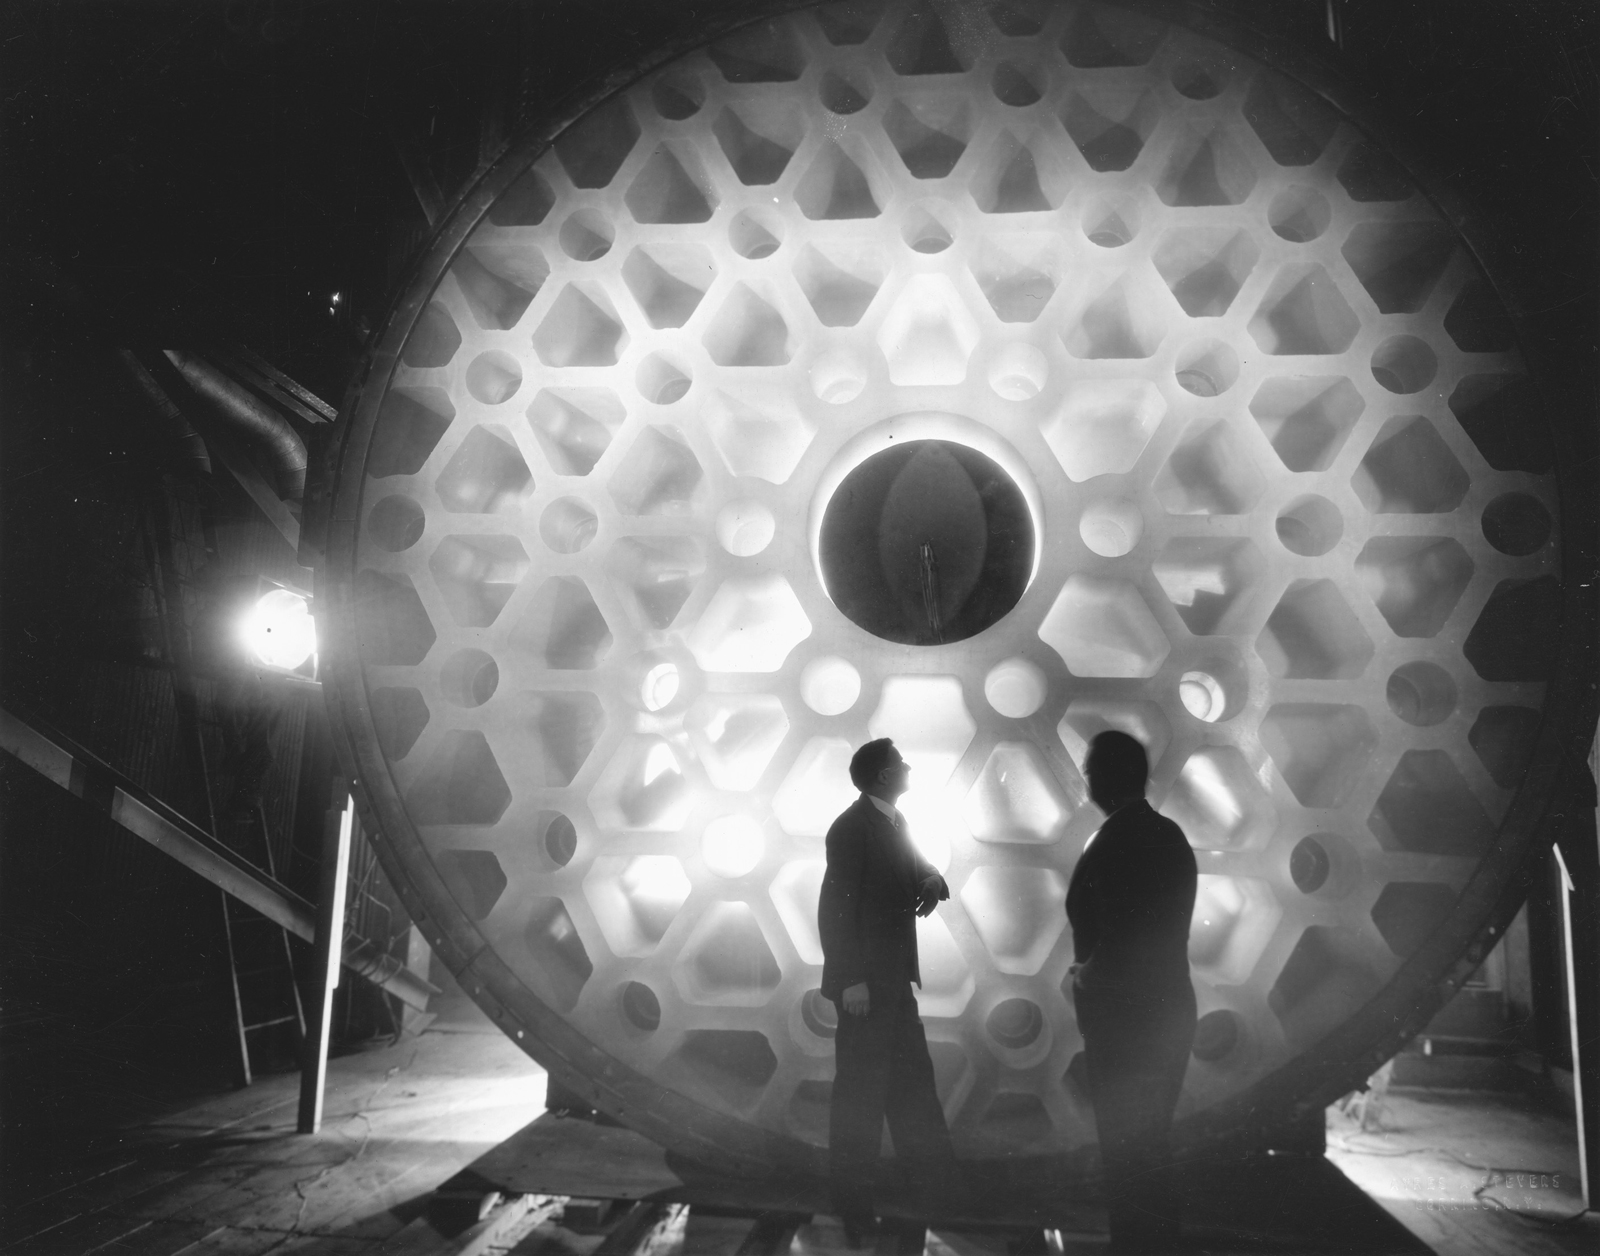
\includegraphics[width=12 cm]{../Figures/twomen}
\caption{Image of the Hale 200-inch (5.1m) primary mirror.  The honeycomb structure was to reduce the mass of the optic and make the surface more ridged}
\label{fig:hale}
\end{figure}

Eventually, these mirrors were becoming so
large that the mirrors would sag under their own weight.  These large optics quickly became heavier and needed
more mechanical supports.  In order to solve this problem, a honeycomb substructure was designed to keep the
mirrors lighter and more ridged.  Figure \ref{fig:hale} shows the primary mirror of the 200-inch Hale telescope
and backlight to show the structure.  While this helped keep large single optics rigid, there is still a limit
to how large one optic can be.  The University of Arizona's Large Optics Facility is capable of constructing
8.4 meter mirrors \cite{LOFTSystems.}.  One of the reasons for this limit is that this is roughly the maximum
width of bridge underpasses in Arizona.  In order to achieve larger primary apertures, a different approach is
needed.




\section{Segmented Mirrors / Active Optics}
\label{sec:seg_mirror}

In 1977, Dr. Jerry Nelson along with Dr. Terry Mast and a team of scientists at the Lawrence Berkeley National Laboratory, were tasked with designing a 10-meter telescope \cite{BeatingObservatory}.  The design they came up with was to use 36, 1.8 meter, hexagonal segments combined to make a 10-meter aperture (Figure \ref{fig:jerry_nelson}).  In order to make this work, all the segments needed to be aligned to sub-wavelength position.  This was accomplished by what is known as active optics.

\begin{figure}[H]
\centering
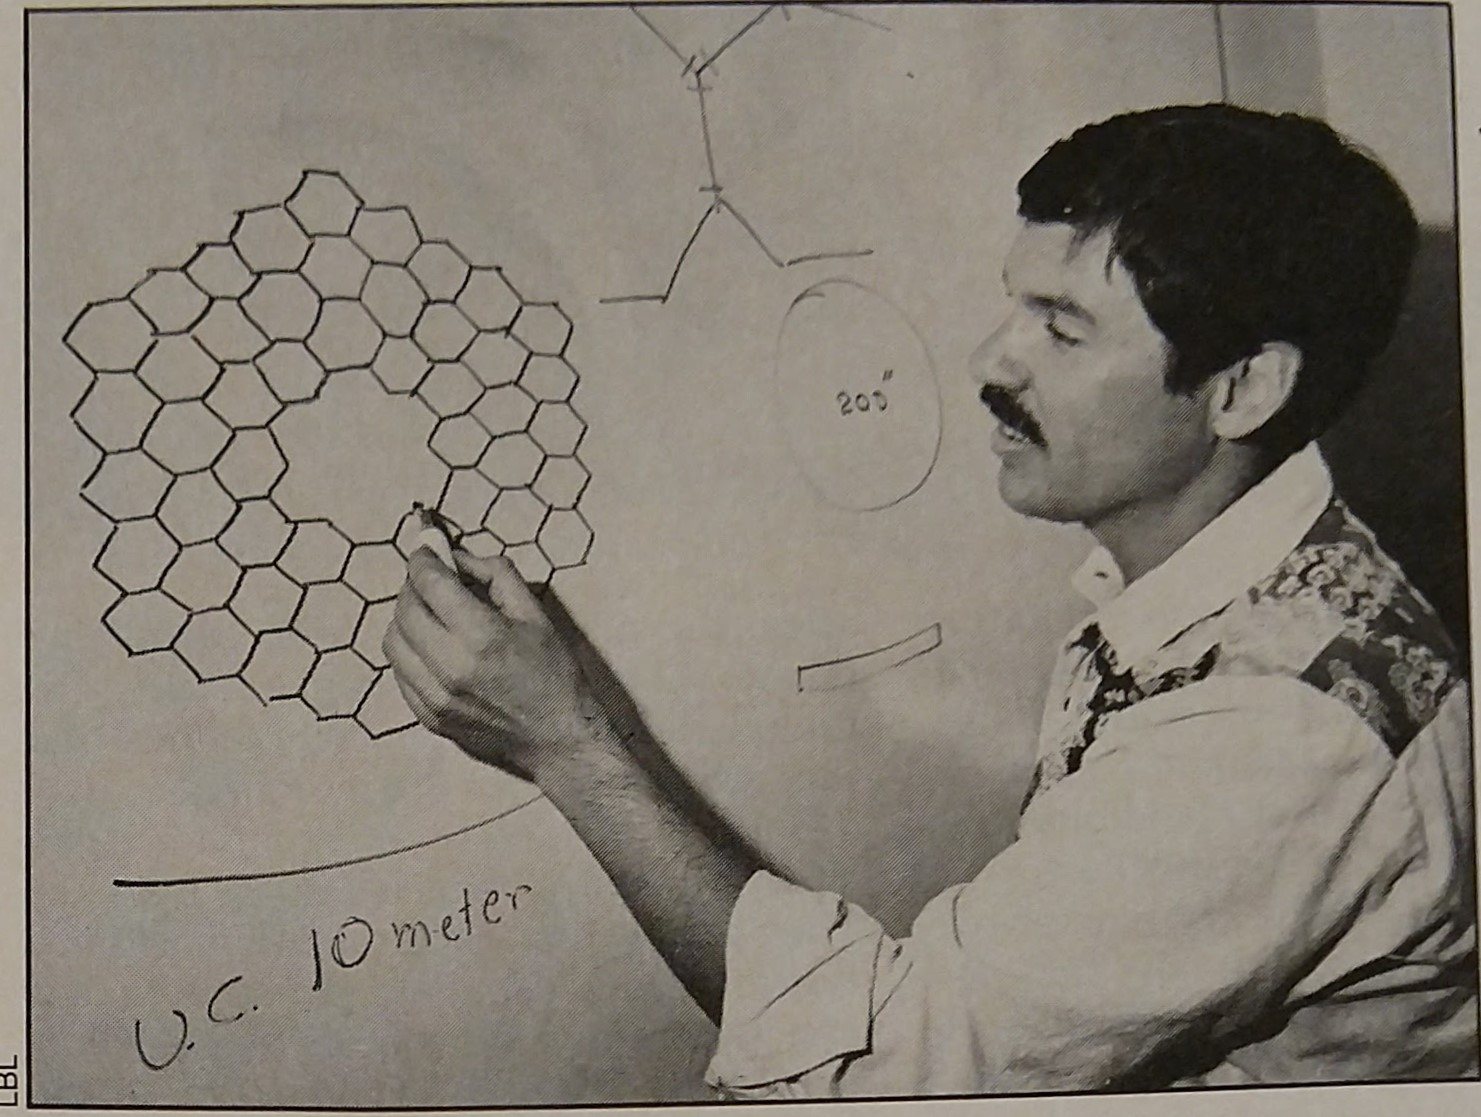
\includegraphics[width=12 cm]{../Figures/Jerry Nelson}
\caption{Jerry Nelson showing his segmented mirror design at Lawrence Berkeley Nation Laboratory.}
\label{fig:jerry_nelson}
\end{figure}

Active optics is the active control of each mirror segment so that all segments act as one large optic.  This is accomplished with nanometer level precision and differential capacitors to measure relative segment movement \cite{Nelson1990titleConstructionObservatory/title}.  This system is continuously running during observation and makes corrections from vibrations that the telescope may experience (i.e mechanical vibration, wind shake, etc).  The Keck position sensors are accurate to $\approx$ 30nm using differential capacitors.  A system view of the the Keck active optics can be seen in Figure \ref{fig:active_control}.


\begin{figure}[H]
\centering
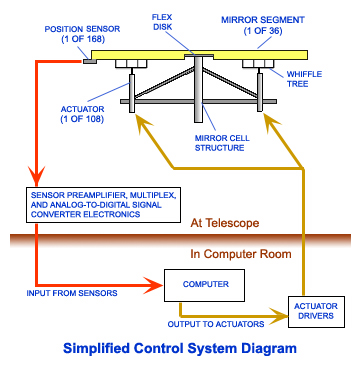
\includegraphics[width=8 cm]{../Figures/KCompDiag}
\caption{A system diagram of the Keck Telescope active control for a segment.}
\label{fig:active_control}
\end{figure}

Instead of hexagonal segments the Giant Magellan Telescope will be using seven, 8.4-meter, circular segments to make up it's 25 meter aperture (Figure \ref{fig:GMT_phase}).  Figure \ref{fig:GMT_phase} shows the initial plan to phase the GMT segments using laser interferometers to detect displacements for both fine and coarse motions \cite{Acton2012PhasingGMT}.  However, these position sensors, like the capacitors, are differential and need to be calibrated.  Typically, a phasing camera with a wavefront sensor is used to phase the mirror segments together.


\begin{figure}[H]
\centering
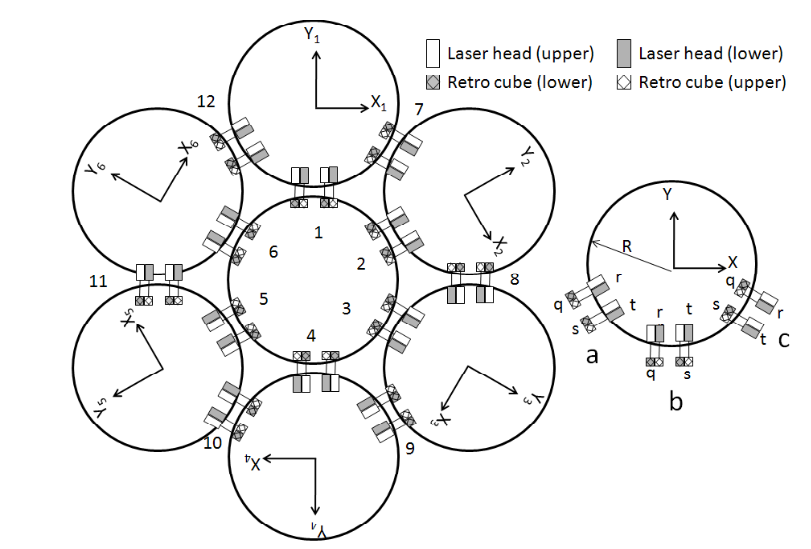
\includegraphics[width=12 cm]{Figures/GMT_phase_measure.png}
\caption{A figure of the GMT pupil and the initial plan to phase the mirrors\cite{Acton2012PhasingGMT}.}
\label{fig:GMT_phase}
\end{figure}


For example, the case of the Keck telescope, there is a seperate instrument all together mounted on a bent Cassegrain port \cite{Chanan1994}.  This camera uses a Shack-Hartmann Wavefront sensonr to measure the piston, tip, and tilt of each segment (Figure \ref{fig:Keck_phase}).  However, for high contrast imaging, this is not an accurate enough way to phase the mirror segments.  High contrast imaging requires as little error as possible in all of the optical systems and the ability to ensure that segments are phased at the focal plane of the camera is highly desireable.  The process of detecting wavefront aberrations in the science images is called Focal Plane Wavefront Sensing (FPWFS).  

\begin{figure}[H]
\centering
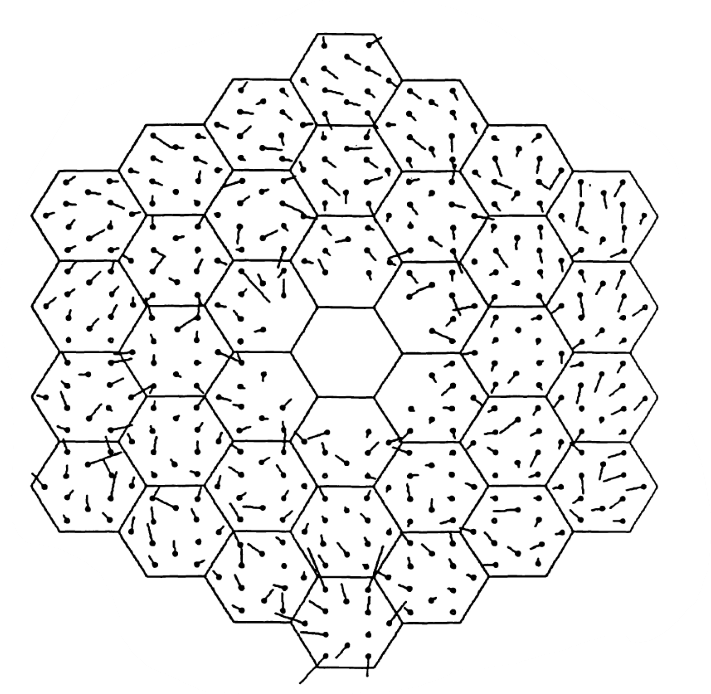
\includegraphics[width=8 cm]{Figures/keck_phasing.png}
\caption{A figure of the spot layout for the Keck phasing camera \cite{Chanan1994}.}
\label{fig:Keck_phase}
\end{figure}


    

\section{FPWFS}
\label{sec:fpwfs}



\subsection{Vector Apodizing Phase Plate}
\label{sec:vAPP}

There are a few different approaches to doing FPWFS, but for this paper we will focus on using a type of coronagraphic imaging optic called a vector apodizing phase plate (vAPP).  A vAPP is a half-wave retarder placed in the pupil-plane.  The apodizing phase plate portion of the optic seperates the right and left handed circular polarization of light and then spatially separated by a phase ramp (Figure \ref{fig:vapp_concept}) \cite{Bos2019Focal-planePlate}.



\begin{figure}[H]
\centering
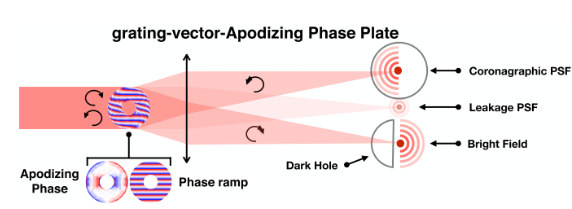
\includegraphics[width=14 cm]{Figures/vAPP.png}
\caption{A conceptual drawing of how a vector apodizing phase plate works \cite{Bos2019Focal-planePlate}.}
\label{fig:vapp_concept}
\end{figure}

The spatial separation after being focused will show in the focal plane as two separate coronagraphic PSF's.  However, the portion of the light that is not polarized will pass through the vAPP unaffected and will show in the focal plane as a standard PSF that can be used for referencing.  But for the purposes of this thesis, we will be looking at the three PSFs and use them to deconstruct phase differences in the segments of the GMT.


\subsection{Asymmetric Pupil}
\label{sec:asym_pupil}

Work and theory done in this section is referenced from Steven Bos's paper \textit{Focal-plane wavefront sensing with the vector Apodizing Phase Plate} \cite{Bos2019Focal-planePlate}.

What makes wavefront sensing possible with a vAPP is the asymmetry that is placed in the pupil plane.  The electric field in the pupil can be written down as:

\begin{align}
    E_{pupil}(r) &= A(r) e^{i \theta(r)} \\
    &= A(r) (\cos[\theta (r)] + i\sin[\theta (r)]
    \label{eq:E_field}
\end{align}

As seen in Equation \ref{eq:E_field}, there is an imaginary component to the electric field.  Propagate this to the focal plane, we get a similar equation only with an added constant of integration.  So this means that only some of the aberrations will appear in our focal plane.  Specifically even phase aberrations will be left out of the focal plane while odd phase aberrations will continue to pass through.  Adding an asymmetry to the pupil plane creates an odd amplitude which generates a real electric field.  The real electric field will interfere with the aberrations' real electric field and will enable detection of the aberration in the focal plane \cite{Bos2019Focal-planePlate}.



\begin{figure}[H]
\centering
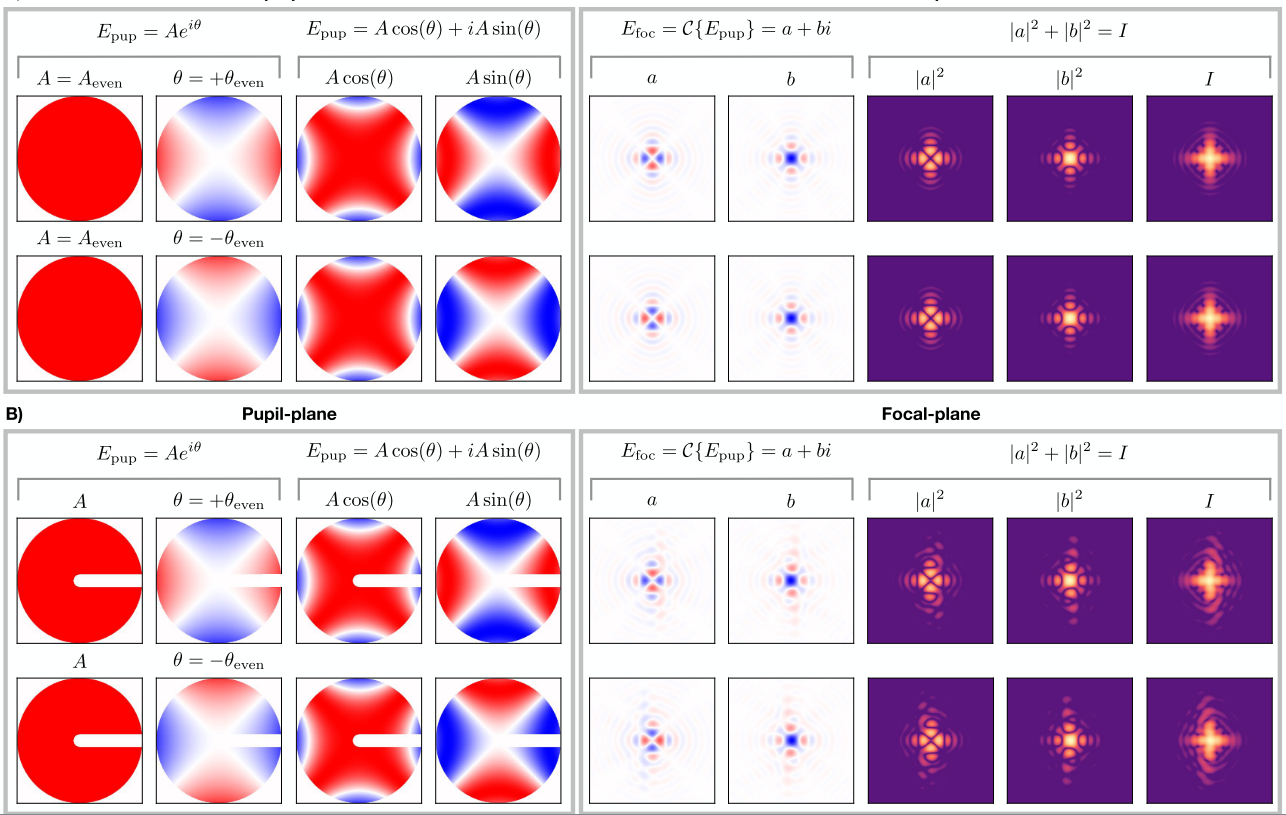
\includegraphics[width=14 cm]{Figures/asymmetry.png}
\caption{Figure showing how adding an asymmetry to the pupil plane propagates even phase aberrations and not through a symmetric pupil plane \cite{Bos2019Focal-planePlate}.}
\label{fig:vapp_concept}
\end{figure}

With the theory in place, we can implement this into showing that using an Asymmetric vector Apodizing Phase Plate can show phase errors in the GMT segments.


%----------------------------------------------------------------------------------------
%	SECTION 1
%----------------------------------------------------------------------------------------
